\section{Цель лабораторной работы}

Изучение и реализация базовых методов планирования эксперимента:
\begin{itemize}
    \item{метод наименьших квадратов (МНК);}
    \item{метод Гаусса решения системы линейных алгебраических уравнений.}
\end{itemize}

\section{Задача лабораторной работы}

В ходе лабораторной работы необходимо реализовать и отладить программу аппроксимирующую экспериментальные данные некоторой плоскостью с помощью метода наименьших квадратов (МНК) и метода Гаусса для решения системы линейных алгебраических уравнений.

\section{Используемые инструменты}

Поставленная задача решалась с использованием следующих инструментов:
\begin{itemize}
    \item{операционная система \href{https://debian.org}{Debain 12};}
    \item{компилятор языка c++ из \href{https://gcc.gnu.org/}{GNU Compiler Collection (gcc)};}
    \item{сборка проекта производилась с помощью утилиты \href{https://cmake.org/}{cmake}.}
    \item{текстовый редактор \href{https://ru.wikipedia.org/wiki/Vim}{vim};}
\end{itemize}

\section{Теоретические основы}

\subsection{Постановка задачи}
Пусть в результате эксперимента получена серия двумерных массивов, элементы которых можно рассматривать, как точки поверхности и необходимо определить координаты максимума выпуклости поверхности.

Особенность задачи состоит в том, что ограничиться определением индекса элемента, имеющего максимальное значение, нельзя, поскольку, во-первых, некоторые поверхности наклонены к горизонтали, и точки на верхнем краю могут быть выше точек на пике выпуклости, во-вторых, могут присутствовать ложные пики.

Решение состоит в том, чтобы выровнять заданную поверхность, аппроксимировав ее плоскостью, а затем из каждой точки поверхности вычесть значение аппроксимирующей функции в данной точке. Далее, выровненную поверхность можно аппроксимировать некоторой поверхностью вращения, например, параболоидом, и найти координаты его максимума~\cite{approximation_plane}.

\subsection{Основыне понятия}

Методы теории планирования экспериментов (ТПЭ) направлены на разработку оптимальных планов проведения экспериментов с целью сокращения объема проводимых исследований при заданной точности и достоверности получения результатов,извлечения из полученных опытных данных максимума полезных сведений.

Исследуемый объект (реальный объект, модель объекта) рассматривается как <<черный ящик>>, имеющий входы $X$ (управляемые независимые параметры) и выходы $Y$.

Переменные $x$ принято называть \emph{факторами}.

Вектор $Y$ называется \emph{откликом}. Зависимость отклика от факторов носит название \emph{функции отклика}, а геометрическое представление функции отклика – \emph{поверхности отклика}. Функция отклика рассматривается как показатель качества или эффективности объекта~\cite{theory_of_plane_experiment}.

\subsection{Метод наименьших квадратов}

Рассмотрим простой случай однофакторного эксперимента. Пусть функция отклика в нашем эксперименте (уравенение регрессии) имеет вид:
\begin{equation}
y = b_0 + b_1 x_1
\end{equation}

Для нахождения функции отклика необходимо определить коэффициенты $b_0$ и $b_1$ по результатам полученных в эксперименте данным. Поскольку не все экспериментальные точки лежат на одной прямой, то можно говорить о наличии $\xi_i$ -- разности между экспериментальным и вычисленным по уравнению регрессии значениями $y$ в $i$-й экспериментальной точке:

\begin{equation}
    y_i - b_0 - b_1 x_1 = \xi_i
\end{equation}

Задача стоит найти такие коэффциенты $b_0$ и $b_1$ при которых отклонения $\xi$ будут минимальны:
\begin{equation}
    U = \sum_{i=1}^{N} \xi_i^2 = \text{min}.
    \label{math:mnk}
\end{equation}

Уравнение~\ref{math:mnk} представляет собой метод наименьших квадратов (МНК). Для получения коэффициентов обязательным условием является наличие не меньшего числа экспериментов над числом неизвестных коэффициентов. Преобразуем уравнение~\ref{math:mnk} к виду:
\begin{equation}
    U = \sum_{i=1}^{N} \xi_i^2 = \sum_{i=1}^{N}(y_i - b_0 - b_1 x_{1,i})^2 =  \text{min}.
    \label{math:mnk_full}
\end{equation}

Известно, что минимум некторой функции, если он существует, достигается при одновременном равенстве нулю частных производных по всем неизвестным, т.е.
\begin{equation}
    \frac{\partial{U}}{\partial{b_0}} = 0, \text{\hspace{2em}}  \frac{\partial{U}}{\partial{b_1}} = 0.
\end{equation}

Взяв частную производную получаем уравнения для определения коэффициентов $b_0$ и $b_1$:
\begin{equation}
    -2 \sum_{i=1}^{N}(y_i - b_0 - b_1 x_{1,i}) = 0, \text{\hspace{2em}} -2 \sum_{i=1}^{N}(y_i - b_0 - b_1 x_{1,i})x_{1,i} = 0.
\end{equation}

Раскрыв скобки и сделав некоторые преобразования получаем:
\begin{equation}
    Nb_0 + \sum_{i=1}^{N}x_{1,i}b_1 = \sum_{i=1}^{N}y_i,  \text{\hspace{2em}} \sum_{i=1}^{N}x_{1,i}b_0 + \sum_{i=1}^{N}x_{1,i}^2 b_1 = \sum_{i=1}^{N}y_i x_{1,i}.
    \label{math:nb0}
\end{equation}

Из уравнения~\ref{math:nb0} можно получить выражения для $b_0$ и $b_1$:
\begin{equation}
    \begin{split}
        b_0 = \frac{\sum\limits_{i=1}^{N}{y_i}\sum\limits_{i=1}^{N}x^2_{1,i} - \sum\limits_{i=1}^{N}{y_i x_{1,i}\sum\limits_{i=1}^{N}x_{1,i}}}{N\sum\limits_{i=1}^{N}{x_{1,i}^2 - \left(\sum\limits_{i=1}^N{x_{1,i}}\right)^2}}, \\[1em]
        b_1 = \frac{N\sum\limits_{i=1}^{N}{y_i x_{1,i}} - \sum\limits_{i=1}^{N}{y_i}\sum\limits_{i=1}^{N}x_{1,i}}{N\sum\limits_{i=1}^{N}{x_{1,i}^2 - \left(\sum\limits_{i=1}^N{x_{1,i}}\right)^2}}.
    \end{split}
\end{equation}

Обобщение на многофакторный случай не связано с какими-либо принципиальными трудностями, но требуют привлеченеия аппарата агебры матриц~\cite{adler_1976}.


\section{Описание алгоритма решения задачи}

Получим систему уравнений для нахождения коэффициентов регрессии для случая двухфакторного эксперимента с помощью МНК.

Функция отклика для случая двухфакторного эксперимента будет иметь следующий вид:
\begin{equation}
    y = b_0 + b_1 x_1 + b_2 x_2,
\end{equation}
где $x_1$, $x_2$ -- факторы в рассматриваемом эксперименте, $b_0$, $b_1$, $b_2$ -- искомые коэффициенты.

Минимизируемая функия суммы квадратов отклонений $U$:
\begin{equation}
    U = \sum_{i=1}^{N}(y_i - b_0 - b_1 x_{1,i} - b_2 x_{2,i})^2 =  \text{min}.
    \label{math:mnk_full}
\end{equation}

Минимум данной функции, если он существует, будет достигаться при одновременном равенстве нулю частных производных по всем неизвестным, т.е.
\begin{equation}
    \frac{\partial{U}}{\partial{b_0}} = 0, \text{\hspace{2em}}  \frac{\partial{U}}{\partial{b_1}} = 0, \text{\hspace{2em}}  \frac{\partial{U}}{\partial{b_2}}  = 0.
\end{equation}


\begin{equation}
    \begin{aligned}
        \frac{\partial{U}}{\partial{b_0}} & = -2 \sum_{i=1}^{N}{(y_i - b_0 - b_1 x_{1,i} - b_2 x_{2,i}) = 2 \sum_{i=1}^{N}{(b_0 + b_1 x_{1,i} + b_2 x_{2,i} - y_i)}} = 0 \\[1em]
        \frac{\partial{U}}{\partial{b_1}} & = -2 \sum_{i=1}^{N}{(y_i - b_0 - b_1 x_{1,i} - b_2 x_{2,i})x_{1,i} = 2 \sum_{i=1}^{N}{(b_0 + b_1 x_{1,i} + b_2 x_{2,i} - y_i)x_{1,i}}} = 0 \\[1em]
        \frac{\partial{U}}{\partial{b_2}} & = -2 \sum_{i=1}^{N}{(y_i - b_0 - b_1 x_{1,i} - b_2 x_{2,i})x_{2,i} = 2 \sum_{i=1}^{N}{(b_0 + b_1 x_{1,i} + b_2 x_{2,i} - y_i)x_{2,i}}} = 0
    \end{aligned}
\end{equation}

Раскрывая скобки и вынося константы за знак суммы, получаем нормальную форму системы линейных уравнений:
\begin{equation}
    \begin{aligned}
        b_0 \sum_{i=1}^{N}{1}       +  b_1 \sum_{i=1}^{N}{x_{1,i}}        + b_2 \sum_{i=1}^{N}{x_{2,i}}         & = \sum_{i=1}^{N}{y_i},            \\[1em]
        b_0 \sum_{i=1}^{N}{x_{1,i}} +  b_1 \sum_{i=1}^{N} x_{1,i}^2       + b_2 \sum_{i=1}^{N}{x_{2,i} x_{1,i}} & = \sum_{i=1}^{N} {y_i x_{1,i}},   \\[1em]
        b_0 \sum_{i=1}^{N}{x_{2,i}} +  b_1 \sum_{i=1}^{N}{x_{1,i}x_{2,i}} + b_2\sum_{i=1}^{N}{x_{2,i}^2}        & = \sum_{i=1}^{N}{y_i x_{2,i}}.
    \end{aligned}
    \label{math:mnk2}
\end{equation}

После подстановки в~\ref{math:mnk2} данных эксперимента $x_{1,i}$, $x_{2,i}$ и $y_i$ для всех $N$ измерений данную систему можно решить методом Гауса для нахождения искомых коэффциентов $b_0$, $b_1$, $b_2$. Алгоритм метода Гаусса представлен на рис.~\ref{fig:Gauss}.

\begin{figure}[h!]
    \centering
    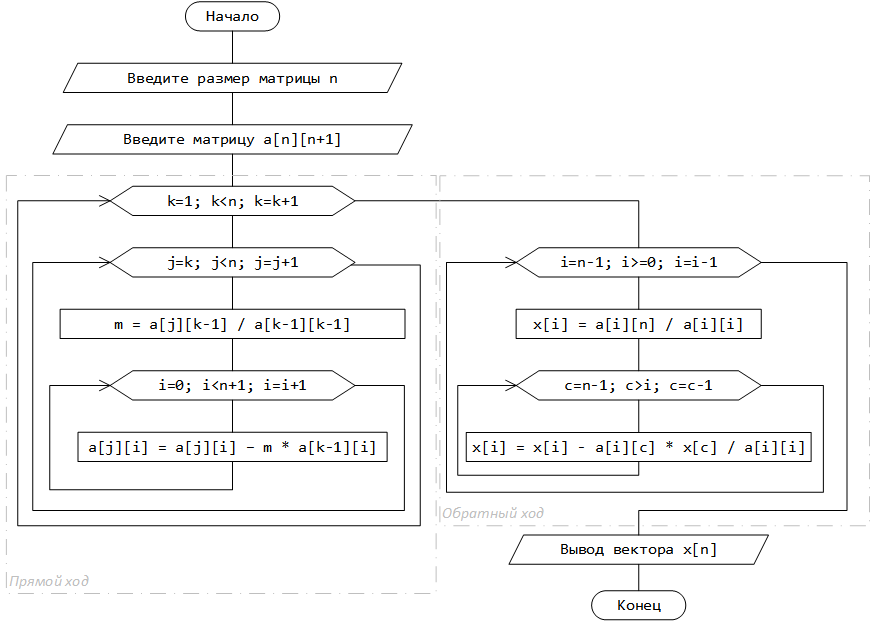
\includegraphics[width=0.75\textwidth]{fig-01}
    \caption{Алгоритм Гаусса для решения системы линейных алгебраических уравнений}
    \label{fig:Gauss}
\end{figure}


\subsection{Метод Гаусса}
Метод Гаусса — классический метод решения системы линейных алгебраических уравнений. Рассмотрим систему линейных уравнений с действительными постоянными коэффициентами:

\begin{equation}
    \begin{cases}
        a_{11} \cdot x_{11} + a_{12} \cdot x_2 + \dots + a_{1n} \cdot x_n = y_1,
        \\
        a_{21} \cdot x_{21} + a_{22} \cdot x_2 + \dots + a_{2n} \cdot x_n = y_2,
        \\[0.5em]
        a_{n1} \cdot x_{n1} + a_{n2} \cdot x_2 + \dots + a_{nn} \cdot x_n = y_n.
     \end{cases}
\end{equation}

Метод Гаусса решения системы линейных уравнений включает в себя 2 стадии:
\begin{itemize}
    \item{последовательное (прямое) исключение;}
    \item{обратная подстановка.}
\end{itemize}

Исключения Гаусса основаны на идее последовательного исключения переменных по одной до тех пор, пока не останется только одно уравнение с одной переменной в левой части. Затем это уравнение решается относительно единственной переменной. Таким образом, систему уравнений приводят к треугольной (ступенчатой) форме. Для этого среди элементов первого столбца матрицы выбирают ненулевой (а чаще максимальный) элемент и перемещают его на крайнее верхнее положение перестановкой строк. Затем нормируют все уравнения, разделив его на коэффициент $a_{i1}$, где $i$– номер столбца.

\begin{equation}
    \begin{cases}
        x_{11} + \frac{a_{12}}{a_{11}} \cdot x_2 + \dots + \frac{a_{1n}}{a_{11}} \cdot x_n = \frac{y_1}{a_{11}},
        \\
        x_{11} + \frac{a_{22}}{a_{21}} \cdot x_2 + \dots + \frac{a_{2n}}{a_{21}} \cdot x_n = \frac{y_2}{a_{21}},
        \\[0.5em]
        x_{11} + \frac{a_{n2}}{a_{n1}} \cdot x_2 + \dots + \frac{a_{nn}}{a_{n1}} \cdot x_n = \frac{y_1}{a_{n1}},
     \end{cases}
\end{equation}

Затем вычитают получившуюся после перестановки первую строку из остальных строк:

\begin{equation}
    \begin{cases}
        x_{11} + \frac{a_{12}}{a_{11}} \cdot x_2 + \dots + \frac{a_{1n}}{a_{11}} \cdot x_n = \frac{y_1}{a_{11}},
        \\[0.3em]
        0 + \left(\frac{a_{22}}{a_{21}} - \frac{a_{12}}{a_{11}} \right) \cdot x_2 + \dots + \left(\frac{a_{2n}}{a_{21}} - \frac{a_{1n}}{a_{11}}  \right) \cdot x_n = \frac{y_2}{a_{21}},
        \\[0.7em]
        0 + \left(\frac{a_{n2}}{a_{n1}} - \frac{a_{12}}{a_{11}} \right) \cdot x_2 + \dots + \left( \frac{a_{nn}}{a_{n1}} - \frac{a_{1n}}{a_{11}}  \right) \cdot x_n = \frac{y_1}{a_{n1}},
     \end{cases}
\end{equation}

Получают новую систему уравнений, в которой заменены соответствующие коэффициенты:

\begin{equation}
    \begin{cases}
        x_{11} + a_{12}'\cdot x_2 + \dots + a_{1n}' \cdot x_n = y_1',
        \\
        0 + a_{22}' \cdot x_2 + \dots + a_{2n}' \cdot x_n = y_2',
        \\[0.5em]
        0  + a_{n2}' \cdot x_2 + \dots + a_{nn}' \cdot x_n = y_n'.
     \end{cases}
\end{equation}

После того, как указанные преобразования были совершены, первую строку и первый столбец мысленно вычёркивают и продолжают указанный процесс для всех последующих уравнений пока не останется уравнение с одной неизвестной:

\begin{equation}
    \begin{cases}
        x_{11} + a_{12}'\cdot x_2 + \dots + a_{1n}' \cdot x_n = y_1',
        \\
        0 +  x_2 + \dots + a_{2n}'' \cdot x_n = y_2'',
        \\
        \dots
        \\
          0 + 0 + \dots +x_n = y_n^{n'}.
     \end{cases}
\end{equation}

Обратная подстановка предполагает подстановку полученного на предыдущем шаге значения переменной $x_n$ в предыдущие уравнения~\cite{gaus_cpp}.

\section{Листинг программы МНК}

\begin{small}
    %// \begin{lstlisting}[language=c++]
        \lstinputlisting[language=c++,firstline=3, lastline=130]{code/mnk.cpp}
    %\end{lstlisting}
\end{small}
